\subsection{EFT intereprations}

Effective Field Theory (EFT) is an model independent way to parametrize the high enregy scale effects in the enregy scale available to us. The general form of the lagrangian is:

\begin{equation}
    \mathcal{L} = \mathcal{L}_{SM} + \mathcal{L}^{5} + \mathcal{L}^{6} + \mathcal{L}^{7} + \ldots,\quad \mathcal{L}^{(d)} = \sum_{i=1}^{n_d} \frac{C_i^{(d)}}{\Lambda^{d-4}}Q_i^{(d)} \quad \textrm{for}~ d>4,
\end{equation}

Where $\Lambda$ is the New Physics (NP) enregy scale, the parameter $C_{i}{(d)}$ are the Wilson Coefficients.

One of most promissing EFT model is the SMEFT \cite{Brivio:2017btx,Aebischer:2017ugx}. Since the operators $Q_{i}^{(d)}$ are surpresssed by the power of cutoff scale $\Lambda$, so we will work with dimension-6 operators only.

Currently, we are trying to produce the Leading Order (LO) ggH process with additional jets upto 2 jets. Like:

\begin{verbatim}
import model SMEFTsim_A_general_MwScheme_UFO_v2
#import model SMEFTsim_A_general_alphaScheme_UFO_v2
generate p p > h QED=1 NP<=1 @0
add process p p > h j QED=1 NP<=1 @1
add process p p > h j j QED=1 NP<=1 @2
\end{verbatim}

Our plan with this is following:

\begin{itemize}
    \item Generate SM from the SMEFT model and compare it with the NNNLOPS official samples (from HIG-19-001).
    \item Decide the set of parameter for which our analysis is sensitive.
    \item Validate the reweight method for our model.
    \item After finalizing previous step we will try to submit for official full CMSSW simulation.
\end{itemize}

\subsection{Additionnal Prediction}
In order to do the additional cross check, we also exploite the ggH sample predicted by MadGraph5_aMCatNLO with NLO QCD accuracy for zero, one and two additional partons merged with the FxFx merging scheme and then use for the comparisons with TH predictions.

HC_NLO_X0_UFO-heft \cite{arXiv:1306.6464,P. Artoisenet, P. de Aquino, F. Demartin, R. Frederix, S. Frixione, F. Maltoni, M. K. Mandal, P. Mathews, K. Mawatari, V. Ravindran, S. Seth, P. Torrielli, M. Zaro, "A framework for Higgs characterisation" (JHEP11(2013)043).} is a model file for the characterisation of the boson recently discovered at the LHC.

The effective field theory consists of the SM (except for the Higgs itself), expressed through the physical degrees of freedom present below the EWSB scale, plus a new bosonic state X(JP) with spin/parity assignments JP = 0+, 0−, 1+, 1−, and 2+. 

\begin{equation} 
    \mathcal{L}_{HC,J} = \mathcal{L}_{SM-H} + \mathcal{L}
\end{equation} 

Currently, we produce the Next Leading Order (NLO) ggH process with additional jets up to 2 jets. Like:

\begin{verbatim}
set low_mem_multicore_nlo_generation True
#special model for gluon fusion higgs at NLO (effective theory in infinite top mass limit)
#note that this model is NOT needed for other SM higgs production modes
import model HC_NLO_X0_UFO-heft
define p = g u c b d s u~ c~ d~ s~ b~
define j = g u c b d s u~ c~ d~ s~ b~
generate p p > x0 / t a [QCD] @0
add process p p > x0 j / t a [QCD] @1
add process p p > x0 j j / t a [QCD] @2
\end{verbatim}

Here is our djr plots to check the FxFx merging quality.
\begin{figure}[!h] 
\centering 
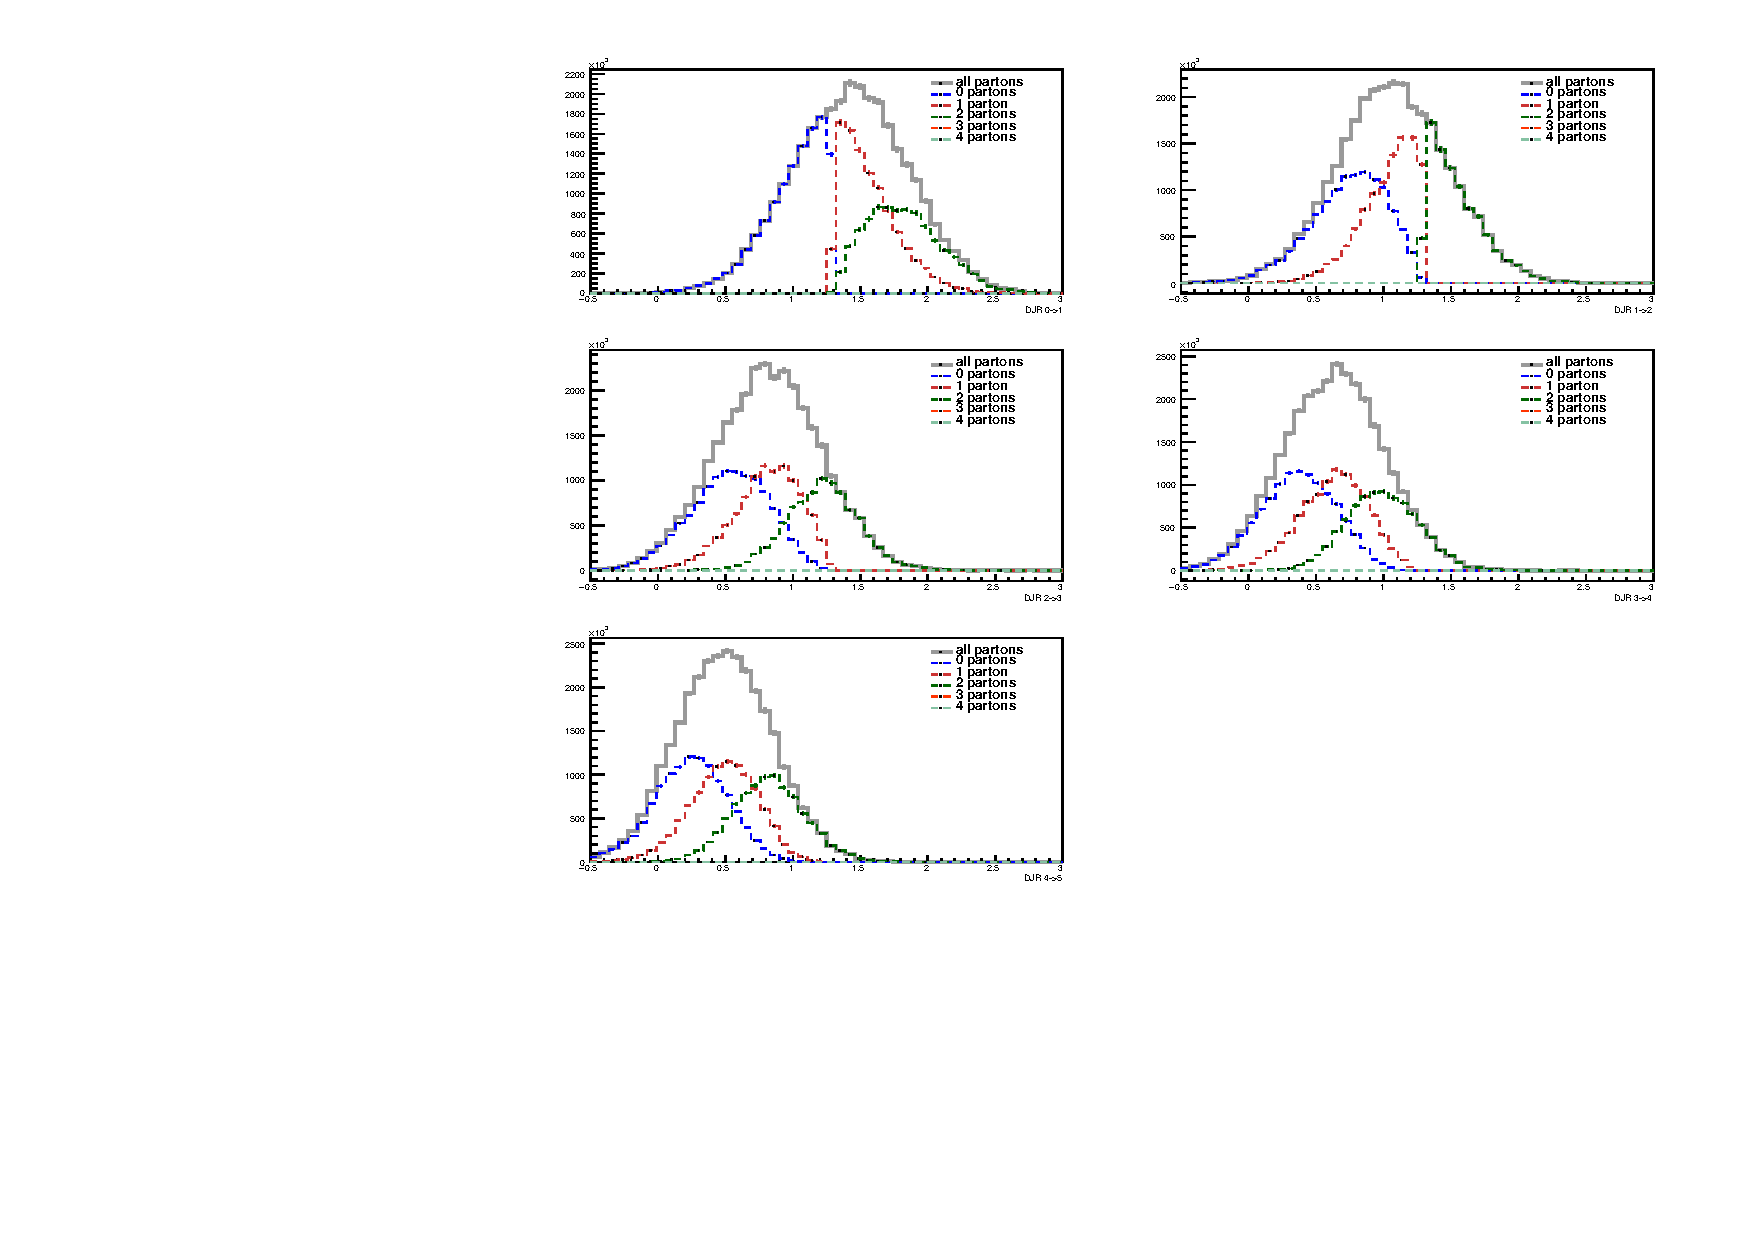
\includegraphics[width=0.32\linewidth]{Figures/EFT/djr_ggh012jToZZTo4LWithOutTau_HC_NLO_heft_5f_NLO_M125_amcatnloFXFX_pythia8_qcut20.pdf}
\caption{Differential Jet Ratio plots for the ggH with additional 0,1,2 jets using HC_NLO_X0_UFO-heft model with FxFx merging. The setting of qCut is 20.}
\label{fig:DJR plots}}  
\end{figure}
